\documentclass[11pt]{article}
\usepackage{setspace}
\setstretch{1}
\usepackage{amsmath,amssymb, amsthm}
\usepackage{graphicx}
\usepackage{bm}
\usepackage[hang, flushmargin]{footmisc}
\usepackage[colorlinks=true]{hyperref}
\usepackage[nameinlink]{cleveref}
\usepackage{footnotebackref}
\usepackage{url}
\usepackage{listings}
\usepackage[most]{tcolorbox}
\usepackage{inconsolata}
\usepackage[papersize={8.5in,11in}, margin=1in]{geometry}
\usepackage{float}
\usepackage{caption}
\usepackage{esint}
\usepackage{url}
\usepackage{enumitem}
\usepackage{subfig}
\usepackage{wasysym}
\newcommand{\ilc}{\texttt}
\usepackage{etoolbox}
\usepackage{algorithm}
\usepackage{changepage}
% \usepackage{algorithmic}
\usepackage[noend]{algpseudocode}
\usepackage{tikz}
\usetikzlibrary{matrix,positioning,arrows.meta,arrows}
\patchcmd{\thebibliography}{\section*{\refname}}{}{}{}
% \PassOptionsToPackage{hyphens}{url}\usepackage{hyperref}

\providecommand{\myceil}[1]{\left \lceil #1 \right \rceil }
\providecommand{\myfloor}[1]{\left \lfloor #1 \right \rfloor }


\begin{document}



\title{\textbf{CSDS 455: Homework 6}}

\author{Shaochen (Henry) ZHONG, \ilc{sxz517}}
\date{Due and submitted on 09/14/2020 \\ Fall 2020, Dr. Connamacher}
\maketitle

\section*{Problem 1}

\begin{proof}
We have $rad(G) \leq diam(G)$ proven by definition. Now locate vertices $u, v \in V(G)$ with $diam(G) = d(u, v)$, then locate a vertex $c$ to the center of $G$. We know that $diam(G) = d(u, v) \leq d(u, c) + d(c, v) \leq 2\epsilon(c)$. Due to the nature of $c$ being a center vertex, we also know that any vertex has a $\epsilon(c) = rad(G)$ by definition, thus we have $diam(G) \leq 2rad(G)$ and the statement is proven by direct proof.
\end{proof}

\section*{Problem 2}

\begin{proof}

The question is essentially same as proving that the \textsc{Prim}'s algorithm produced tree $P$ is a minimum weight spanning tree of $G$. This is because if $T$ is a minimum weight spanning tree of $G$ with a weight of $W$, by doing the equal-weight-edge-replacements on $T$ to make $T', T'', T'''$... we will eventually have a replaced version of $T$ that is same as $P$, as both $T$ and $P$ (if being a minimum weight spanning tree of $G$) have a weight of $W$.

\leavevmode\newline


    \begin{adjustwidth}{1cm}{}

    \textbf{Lemma (Cut Property): Assume $S \in V(G)$ with $G$ being a graph with distinct edge weights. If the minimum cost edge between $V-S$ and $S$ is $e$, this edge $e$ must be contained in the minimum weight spanning tree of $G$}.\newline
    \begin{proof}
    To prove by contradiction: Denote the minimum weight spanning tree of $G$ to be $M$ and assume edge $e$ is not in it. This means there must be some other edge $e'$ that connects $V$ to $V-S$. Since we know that $w(e) < w(e')$ and $M$ is connected, $M - e' + e'$ will another spanning tree of $G$ and has a lower weight. This contradicts the assumption of $M$ being a minimum weight spanning tree of $G$, and the statement is therefore proven.
    \end{proof}
    \end{adjustwidth}

With the lemma proven. Now assume $P$ is not a minimum weight spanning tree of $G$ and traverse through the sequences of vertices of $P$ and $T$. Let $P_{k+1} \subseteq P$ denotes the first tree that has an edge that is not contained in $T$ (as in $P$, it went from its $k$-th vertex $x$ to $(k+1)$-th vertex $y$; but in $T$, it went from its $k$-th vertex $x$ to $(k+1)$-th vertex $z$). \newline

Now we denotes $P_k = P_{k+1} - y$, and edge $<x, y>$ to be the minimum edge from $P_k$ to $V - P_k$ (as it is defined by the mechanism of \textsc{Prim}'s algorithm). By lemma, this edge $<x, y>$ must be in the minimum weight spanning tree $T$. However, $<x, y>$ is not in $T$ as $T$ should chose edge $<x, z>$. This contradicts the setting and our assumption of $P$ is not a minimum weight spanning tree of $G$ is therefore voided.

Since at the beginning we have estalished that proving $P$ to be a minimum weight spanning tree of $G$ is equivalent to the proposed statement. The statment is therefore proven.\newline

Note the lemma is proved based on the assumption of a graph having distinct edge weights. However, this may not be true for the proposed $G$. Which would suggest a minimal cost edge $e$ may not been chosen to connect $V$ to $V-S$ as an alternative edge $e''$ with $w(e'') = w(e)$ is chosen. However, this won't effect the conclusion as as long as $P$ has the same weight of a minimum weight spanning tree, we may convert $T$ to $P$ by doing the equal-weight-edge-replacement manuver.

\end{proof}

\section*{Problem 3}

\begin{proof}

    To prove by counterexample: Assume we have the graph directed graph with negative edge weight of the following.

    \begin{figure}[H]
        \centering
        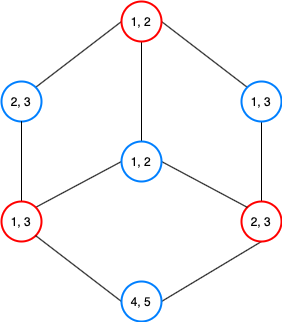
\includegraphics[width=0.3\linewidth]{{fig/fig_p3.png}}
        \label{fig:1}
    \end{figure}

    Staring from $S$ as the source, the first iteration of \textsc{Dijkstra}  will give us $S{0}; \ X: {5, S}; \ Y: {1, S}$ with $S$ removed from unvisited nodes. As $Y$ has the shortest cost from all unvisited nodes, we will start our second iteration from $Y$. Which will give us the same $S{0}; \ X: {5, S}; \ Y: {1, S}$, as $Y$ has no neighbor, with $X, Y$ removed from unvisited nodes. Now we start our third iteration with our only unvisited node $X$, since there are no other unvisited node, the iteration will stop with the same $S{0}; \ X: {5, S}; \ Y: {1, S}$.\newline

    This \textsc{Dijkstra}'s algorithm produce a spanning tree of node sequence of $\{ <S, Y>, <S, X> \}$ with a total tree weight of $5 + 1 = 6$. However, the actual shortest spanning tree should be $\{<S, X>, <X, Y>\}$ with a tree weight of $5 - 10 = -5$. As $-5 < 6$, this counterexample has proven the statement.

\end{proof}


\section*{Problem 4}

\textit{For this quetion I have consulted \url{https://www.cs.cmu.edu/~ckingsf/class/02713-s14/lectures/lec11-bellman.pdf}.}


\begin{proof}

It is my understaning that I can produce a spanning tree of $G$ with the \textsc{Bellman-Ford} algorithm. The detail procedure of such algorithm is omitted, but the general principle is from source node $s$, we set $d(s) = 0$ and $d(v) = \infty$ for all $v \in V(G) - s$. Then we find an edge $(u, v)$ where $d(u) + d(u, v) < d(v)$ and set $d(v) = d(u) + d(u,v)$, until we have $d(u) + d(u, v) \geq d(v)$ for every possible $u, v$ pair in $V(G)$. We denotes the tree generated by this algorithm as $T$.\newline

We want to show that for any arbitrarily selected $v \in V(G)$, there should be $w(P_{sv}) \geq d_T(v)$, where $P_{sv}$ can be any path from $s$ to $v$.  We will show this be using induction on number of edges in $P_{sv}$.

For $n = 1$, the assumption is trivially true as there is only one egde from $s$ to $v$ in $G$, so of course there is $w(P_sv_1) = d_T(v)$. Assume this is also true for $k$ edges: which means if the last of $k$-edged $P_{sv}$ is $v_k$, we have $w(P_{sv_k}) \geq d_T(v_k)$.

Now let $P_{sv_{k+1}}$ to be a path with $k+1$ edges, where $P_{sv_{k+1}} = P_{sv_k} + (v_k, v_{k+1})$. There must be:

\begin{equation*}
    w(P_{sv_{k+1}}) = w(P_{sv_k}) + d(v_k, v_{k+1}) \geq d_T(v_k) + d(v_k, v_{k+1}) \geq d_T(v_{k+1})
\end{equation*}

As otherwise we void the $d(u) + d(u, v) \geq d(v)$ requirement and should keep iterating the \textsc{Bellman-Ford} algorithm with more \textsc{Ford} step(s). As $v_k$ and $v_{k+1}$ can be any two adjacent nodes in $V(G) - s$, and with the statement of $w(P_{sv_k}) \geq d_T(v_k)$ to be true for both $1$, $k$, and $k+1$ cases, we have proven the statement to be true.

\end{proof}

% \section{References}
%
% \nocite{*}
% \raggedright
% \bibliography{references.bib}
% \bibliographystyle{plain}


\end{document}